\chapter{La catalyse homogène dans l'industrie}\label{ch:b3:homogeneous-catalysis}

La plus grande partie de l'acide acétique mondial, matière première de
l'acétate de vinyle, de l'acétate de cellulose et de l'acide téréphtalique
purifié des bouteilles en plastique, est fabriquée à partir de méthanol et
de monoxyde de carbone dans quelques très grandes usines. Dans chacune, un
complexe du rhodium ou de l'iridium, dissous à faible concentration dans le
liquide réactionnel, accomplit des milliers de cycles par heure, pendant
des années. La même chimie hydrogène, additionne CO et dihydrogène sur les
alcènes, échange les extrémités des doubles liaisons, relie des cycles
aromatiques et produit le polyéthylène et le polypropylène par millions de
tonnes. Ce chapitre lit les cycles catalytiques des principaux procédés
industriels avec les outils du \cref{ch:b3:organometallic-bonding}~:
décomptes d'électrons, degrés d'oxydation, étapes cinétiquement
déterminantes, et symétrie du catalyseur qui fixe la structure d'un
polymère.

\begin{recall}
Le volume de deuxième année a présenté les actes élémentaires des réactions
organométalliques (addition oxydante, élimination réductrice, insertion
migratoire, élimination d'hydrure en $\beta$, transmétallation), les cycles catalytiques,
les précatalyseurs, le nombre de cycles et la fréquence de cycles, et a lu
les cycles de l'hydrogénation, de l'\omterm{def:b3:homogeneous-catalysis:hydroformylation}{hydroformylation} et des couplages
croisés~; il a aussi défini la tacticité et la polymérisation en chaîne, le
taux de conversion et la sélectivité. Le
\cref{ch:b3:organometallic-bonding} a décompté les électrons et décrit les
ligands carbonyle et \omterm{def:b3:organometallic-bonding:carbene}{carbène}~; le \cref{ch:b3:complex-kinetics} a donné la
cinétique de saturation~; le \cref{ch:b3:point-groups}, les \omterm{def:b3:point-groups:operation}{éléments de
symétrie} des molécules.
\end{recall}

\begin{omfigure}
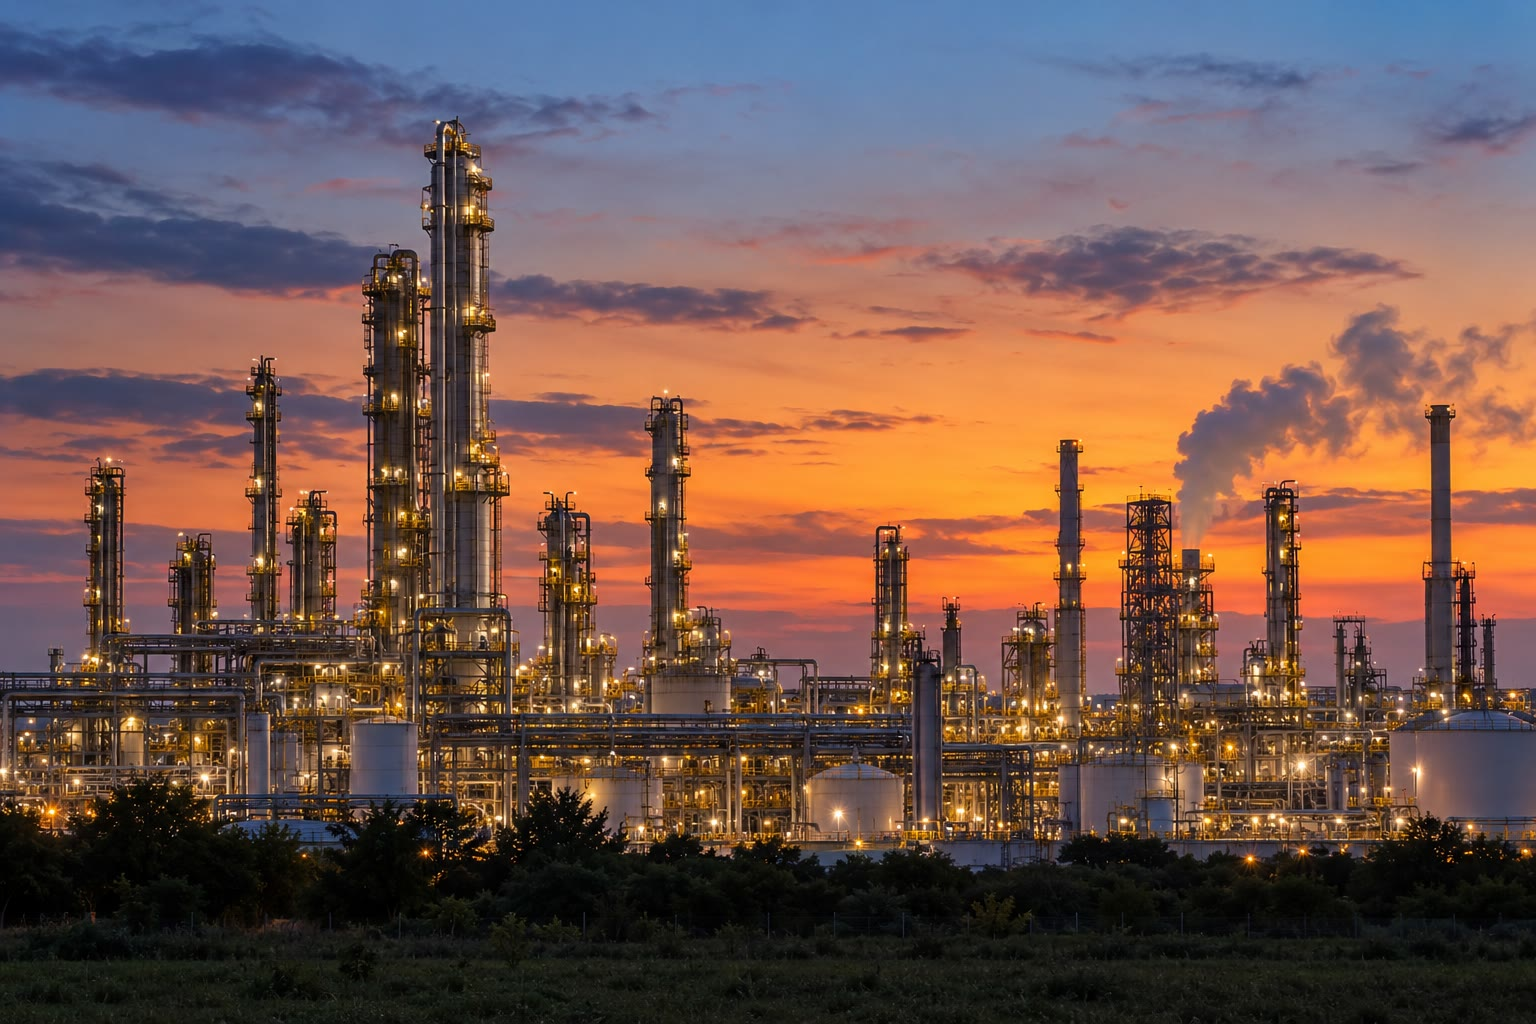
\includegraphics[width=0.6\linewidth]{images/book4/ai/b3-21-chemical-plant.jpg}

{\small Une grande usine chimique au crépuscule. Dans une unité de
\omterm{def:b3:homogeneous-catalysis:carbonylation}{carbonylation}, le catalyseur est un complexe métallique dissous dans le
liquide réactionnel~; l'essentiel de l'usine sert à séparer et à recycler.}
\end{omfigure}

\section{Hydrogénation}

\begin{method}[Lire un cycle catalytique]\label{met:b3:homogeneous-catalysis:read-cycle}
\begin{enumerate}
  \item Pour chaque espèce, compter les électrons de valence et donner le
        degré d'oxydation et le $d^n$ du métal.
  \item Nommer chaque étape (perte ou addition de ligand, addition
        oxydante, insertion, élimination) et vérifier que les décomptes
        varient comme elle l'exige (addition oxydante~: $+2$ pour le degré
        d'oxydation et pour le décompte d'électrons).
  \item Identifier l'état de repos (l'espèce qui s'accumule) et l'étape
        cinétiquement déterminante~; la loi de vitesse découle des
        pré-équilibres qui les relient.
\end{enumerate}
\end{method}

\begin{omfigure}
\begin{tikzpicture}[font=\small, >=Stealth]
  \node (a) at (90:2.3) {\ce{RhCl(PPh3)2} \ (14, Rh$^{\mathrm I}$)};
  \node (b) at (0:3.0) {\ce{RhClH2(PPh3)2} \ (16, Rh$^{\mathrm{III}}$)};
  \node (c) at (-90:2.3) {\ce{RhClH2(RCH=CH2)(PPh3)2} \ (18)};
  \node (d) at (180:3.1) {\ce{RhClH(CH2CH2R)(PPh3)2} \ (16)};
  \draw[->, thick] (a) to[bend left=22] node[midway, above right, font=\scriptsize] {$+\,\ce{H2}$, addition oxydante} (b);
  \draw[->, thick] (b) to[bend left=22] node[midway, below right, font=\scriptsize] {$+$ alcène} (c);
  \draw[->, thick] (c) to[bend left=22] node[midway, below left, font=\scriptsize] {insertion migratoire} (d);
  \draw[->, thick] (d) to[bend left=22] node[midway, above left, font=\scriptsize, align=right] {élimination\\ réductrice~: $-$ alcane} (a);
  \node[anchor=south] (p) at (90:3.4) {\ce{RhCl(PPh3)3} \ (16, précatalyseur)};
  \draw[<->, black!50] (p) -- (a) node[midway, right, font=\scriptsize] {$\mp\,\ce{PPh3}$};
\end{tikzpicture}

{\small Un cycle simplifié de l'hydrogénation des alcènes par le catalyseur
de Wilkinson (décomptes d'électrons de valence entre parenthèses). La perte
d'une phosphine libère un site~; le cycle additionne le dihydrogène, fixe
l'alcène, l'insère dans une liaison Rh--H et élimine l'alcane.}
\end{omfigure}

\begin{proposition}[Cinétique de Wilkinson]\label{prop:b3:homogeneous-catalysis:wilkinson-rate}
Si $\ce{RhClL3} \rightleftharpoons \ce{RhClL2} + \mathrm L$ ($K_1$) et $\ce{RhClL2} + \ce{H2} \rightleftharpoons \ce{RhClH2L2}$ ($K_2$) sont des
équilibres rapides et si la réaction du dihydrure avec l'alcène (constante
de vitesse $k$) est cinétiquement déterminante,
\[
  v = \frac{kK_1K_2[\mathrm{Rh}]_{\mathrm{tot}}[\ce{H2}][\text{alcène}]}{[\mathrm L] + K_1 + K_1K_2[\ce{H2}]},
\]
qui sature en dihydrogène et est inhibée par l'ajout de phosphine L.
\end{proposition}

\begin{proof}
$[\ce{RhClL2}] = K_1[\ce{RhClL3}]/[\mathrm L]$ et $[\ce{RhClH2L2}] = K_2[\ce{H2}][\ce{RhClL2}]$. En écrivant $[\mathrm{Rh}]_{\mathrm{tot}}$ comme la
somme des trois espèces et en résolvant pour le dihydrure, on obtient $[\ce{RhClH2L2}] =
K_1K_2[\ce{H2}][\mathrm{Rh}]_{\mathrm{tot}}/([\mathrm L] + K_1 + K_1K_2[\ce{H2}])$~; la vitesse est $k$ fois cette concentration et celle
de l'alcène.
\end{proof}

Le catalyseur de Wilkinson hydrogène les alcènes peu encombrés bien plus
vite que les alcènes substitués et laisse intacts les groupes carbonyle~:
c'est la sélectivité d'un centre métallique encombré. Des diphosphines
chirales transforment la même chimie en hydrogénation asymétrique
(\cref{ch:b3:asymmetric-synthesis}).

\section{Procédés de carbonylation}

\begin{definition}[Hydroformylation]\label{def:b3:homogeneous-catalysis:hydroformylation}
L'\emph{hydroformylation}\index{hydroformylation} est l'addition d'un atome
d'hydrogène et d'un groupe formyle (CHO) sur une double liaison C=C, à
partir de $\ce{H2}$ et de CO, qui transforme un alcène en un aldéhyde comportant un
carbone de plus. Le \emph{rapport linéaire/ramifié}\index{rapport lineaire/ramifie@rapport linéaire/ramifié} est le rapport
de l'aldéhyde à chaîne droite à l'aldéhyde ramifié.
\end{definition}

Les premiers procédés utilisaient $\ce{HCo(CO)4}$ vers 150 à \qty{180}{\celsius} et sous de
très hautes pressions. Le rhodium associé à la triphénylphosphine opère vers
\qty{100}{\celsius} et sous des pressions bien plus basses, et donne un
\omterm{def:b3:homogeneous-catalysis:hydroformylation}{rapport linéaire/ramifié} plus élevé~: les phosphines encombrées favorisent
l'insertion qui place le métal sur le carbone terminal. Le propène donne le
butanal, hydrogéné en butan-1-ol ou converti en alcools pour plastifiants.

\begin{definition}[Carbonylation]\label{def:b3:homogeneous-catalysis:carbonylation}
La \emph{carbonylation}\index{carbonylation} est l'introduction d'un groupe
carbonyle dans une molécule par réaction avec le monoxyde de carbone,
catalysée par un complexe métallique via l'insertion migratoire de CO.
\end{definition}

La \omterm{def:b3:homogeneous-catalysis:carbonylation}{carbonylation} du méthanol en acide acétique, $\ce{CH3OH + CO -> CH3COOH}$, se fait sur
le rhodium (procédé Monsanto) ou l'iridium (procédé Cativa) avec l'iodure
de méthyle comme cocatalyseur~: l'iodure d'hydrogène transforme le méthanol
en iodure de méthyle, le métal insère CO dans le groupe méthyle, et
l'iodure d'acétyle formé est hydrolysé, ce qui libère de nouveau HI.

\begin{omfigure}
\begin{tikzpicture}[font=\small, >=Stealth]
  \node (a) at (90:2.1) {$\ce{[M(CO)2I2]-}$ (16)};
  \node (b) at (0:2.9) {$\ce{[CH3M(CO)2I3]-}$ (18)};
  \node (c) at (-90:2.1) {$\ce{[CH3COM(CO)I3]-}$ (16)};
  \node (d) at (180:2.9) {$\ce{[CH3COM(CO)2I3]-}$ (18)};
  \draw[->, thick] (a) to[bend left=22] node[midway, above right, font=\scriptsize, align=left] {$+\,\ce{CH3I}$\\ addition oxydante} (b);
  \draw[->, thick] (b) to[bend left=22] node[midway, below right, font=\scriptsize] {insertion migratoire} (c);
  \draw[->, thick] (c) to[bend left=22] node[midway, below left, font=\scriptsize] {$+$ CO} (d);
  \draw[->, thick] (d) to[bend left=22] node[midway, above left, font=\scriptsize, align=right] {élimination réductrice\\ $-\,\ce{CH3COI}$} (a);
  \node[anchor=north, align=center, font=\scriptsize] at (0,-2.55) {$\ce{CH3COI + H2O -> CH3COOH + HI}$, \quad $\ce{CH3OH + HI -> CH3I + H2O}$};
\end{tikzpicture}

{\small Le cycle de \omterm{def:b3:homogeneous-catalysis:carbonylation}{carbonylation} du méthanol pour $\mathrm M = \mathrm{Rh}$ (Monsanto)~; décomptes
d'électrons de valence entre parenthèses, degré d'oxydation du métal I en
haut, III ailleurs. Avec le rhodium, l'addition oxydante de l'iodure de
méthyle est cinétiquement déterminante. Avec l'iridium (Cativa), elle est
bien plus rapide, l'insertion migratoire est lente, et des \omterm{def:b3:surfaces-catalysis:catalyst-design}{promoteurs} qui
arrachent un iodure à $\ce{[CH3Ir(CO)2I3]-}$ accélèrent l'insertion.}
\end{omfigure}

\begin{proposition}[Loi de vitesse du procédé au rhodium]\label{prop:b3:homogeneous-catalysis:monsanto-rate}
Si l'addition oxydante de l'iodure de méthyle sur $\ce{[Rh(CO)2I2]-}$ est cinétiquement déterminante et
si ce complexe est l'état de repos, $v = k[\mathrm{Rh}]_{\mathrm{tot}}[\ce{CH3I}]$~: ordre zéro par rapport à
CO et au méthanol.
\end{proposition}

\begin{proof}
La vitesse est celle de l'étape lente, $k[\ce{[Rh(CO)2I2]-}][\ce{CH3I}]$, et presque tout le
rhodium est dans l'état de repos. CO n'intervient qu'après l'étape lente, et
le méthanol ne fait que régénérer l'iodure de méthyle, dont la
concentration stationnaire est fixée par l'iodure introduit dans le
réacteur plutôt que par le méthanol.
\end{proof}

L'iridium l'a emporté sur le rhodium dans les nouvelles usines pour des
raisons pratiques~: ses complexes restent en solution à plus faible
teneur en eau, ce qui économise l'énergie de séchage du produit, et ils
donnent moins de sous-produits. La principale réaction parasite des deux
procédés est la réaction du gaz à l'eau, $\ce{CO + H2O -> CO2 + H2}$, catalysée par le même métal, qui
gaspille du monoxyde de carbone.

\section{Métathèse des oléfines}

\begin{definition}[Métathèse des oléfines]\label{def:b3:homogeneous-catalysis:metathesis}
La \emph{métathèse des oléfines}\index{metathese des olefines@métathèse des oléfines} est l'échange des
moitiés alkylidène de deux alcènes, $\mathrm{RCH{=}CHR + R'CH{=}CHR' \rightleftharpoons 2\,RCH{=}CHR'}$, catalysé par
des \omterm{def:b3:organometallic-bonding:carbene}{complexes carbéniques} métalliques via un \emph{métallacyclobutane}\index{metallacyclobutane@métallacyclobutane},
cycle à quatre chaînons formé du métal et de trois carbones. Ses formes
synthétiques sont la \emph{métathèse cyclisante}\index{metathese cyclisante@métathèse cyclisante} (RCM), qui
réunit deux extrémités alcène d'une même molécule en un cycle avec perte
d'éthène, la \emph{polymérisation par métathèse par ouverture de cycle}\index{polymerisation par metathese par ouverture de cycle@polymérisation par métathèse par ouverture de cycle}
(ROMP) des alcènes cycliques tendus, et la \emph{métathèse croisée}\index{metathese croisee@métathèse croisée} entre deux
alcènes différents.
\end{definition}

\begin{definition}[Mécanisme de Chauvin]\label{def:b3:homogeneous-catalysis:chauvin}
Le \emph{mécanisme de Chauvin}\index{mecanisme de Chauvin@mécanisme de Chauvin} de la métathèse est la
cycloaddition $[2+2]$ d'un alcène sur un \omterm{def:b3:organometallic-bonding:carbene}{carbène} métallique, $\mathrm{[M]{=}CHR}$, qui donne un
\omterm{def:b3:homogeneous-catalysis:metathesis}{métallacyclobutane}, suivie de sa cyclorétroaddition dans l'autre sens, qui
libère un nouvel alcène et un nouveau \omterm{def:b3:organometallic-bonding:carbene}{carbène}.
\end{definition}

\begin{omfigure}
\setchemfig{atom sep=2.1em}
\schemestart
\chemfig{M=[:0]CHR}
\+
\chemfig{R'HC=[:0]CHR'}
\arrow{<=>}
\chemfig{M?-[:0]CHR-[:-90]CHR'-[:180]CHR'?}
\arrow{<=>}
\chemfig{M=[:0]CHR'}
\+
\chemfig{RHC=[:0]CHR'}
\schemestop
\par\vspace{10pt}

{\small Le \omterm{def:b3:homogeneous-catalysis:chauvin}{mécanisme de Chauvin}~: un \omterm{def:b3:organometallic-bonding:carbene}{carbène} métallique et un alcène se
combinent en un \omterm{def:b3:homogeneous-catalysis:metathesis}{métallacyclobutane}, qui s'ouvre dans l'autre sens pour
donner un nouveau \omterm{def:b3:organometallic-bonding:carbene}{carbène} et un nouvel alcène. Chaque étape est
renversable~: la métathèse atteint un équilibre, sauf si un produit
s'échappe.}
\end{omfigure}

\begin{proposition}[Déplacer la métathèse cyclisante]\label{prop:b3:homogeneous-catalysis:metathesis-equilibrium}
Pour une cyclisation $\text{diène} \rightleftharpoons \text{cycloalcène} + \ce{C2H4}$, éliminer l'éthène de la
solution rend la réaction totale~; la réaction est favorisée par l'entropie
de libération d'une molécule de gaz.
\end{proposition}

\begin{proof}
À l'équilibre, $K = [\text{cycle}][\ce{C2H4}]/[\text{diène}]$~: si $[\ce{C2H4}]$ est maintenue basse par barbotage ou
mise sous vide, $[\text{cycle}]/[\text{diène}] = K/[\ce{C2H4}]$ croît sans limite. Le nombre de molécules
augmente de un au cours de la réaction, tandis que les liaisons formées et
rompues (une C=C de chaque côté) sont semblables~: $\Delta_rH^\circ \approx 0$ pour un cycle non tendu et $\Delta_rS^\circ > 0$, si bien que $K$ est favorable.
\end{proof}

La ROMP des cycles tendus, comme le norbornène, va dans l'autre sens pour
la raison inverse~: la libération de la tension de cycle compense la perte
d'entropie de translation. Les \omterm{def:b3:organometallic-bonding:carbene}{carbènes} du ruthénium de Robert Grubbs
tolèrent l'eau, l'air et la plupart des groupes fonctionnels~; les
alkylidènes du molybdène et du tungstène de Richard Schrock sont plus
actifs et peuvent être rendus énantiosélectifs.

\section{Couplages croisés au palladium}

\begin{definition}[Réactions de couplage croisé]\label{def:b3:homogeneous-catalysis:cross-coupling}
Une \emph{réaction de couplage croisé}\index{reaction de couplage croise@réaction de couplage croisé} relie deux
fragments carbonés différents, un halogénure organique et un réactif
organométallique ou un alcène, sur un catalyseur métallique, le plus souvent
le palladium. Dans la \emph{réaction de Heck}\index{reaction de Heck@réaction de Heck}, un halogénure d'aryle ou de
vinyle se couple avec un alcène pour donner un alcène substitué~; dans le
\emph{couplage de Suzuki--Miyaura}\index{couplage de Suzuki--Miyaura}, il se couple avec un composé
organoboré en présence d'une base.
\end{definition}

\begin{omfigure}
\begin{tikzpicture}[font=\small, >=Stealth]
  \node (a) at (90:2.0) {$\mathrm{Pd^0L_2}$};
  \node (b) at (0:2.6) {$\mathrm{ArPd^{II}XL_2}$};
  \node (c) at (-90:2.0) {$\mathrm{ArPd^{II}Ar'L_2}$};
  \draw[->, thick] (a) to[bend left=25] node[midway, above right, font=\scriptsize, align=left] {$+\,$ArX\\ addition oxydante} (b);
  \draw[->, thick] (b) to[bend left=25] node[midway, below right, font=\scriptsize, align=left] {$+\,\mathrm{Ar'B(OH)_2}$, base\\ transmétallation} (c);
  \draw[->, thick] (c) to[bend left=35] node[midway, left, font=\scriptsize, align=right] {élimination réductrice\\ $-\,$Ar--Ar$'$} (a);
\end{tikzpicture}

{\small Le cycle de Suzuki--Miyaura~: le palladium(0) s'insère dans la
liaison C--X de l'halogénure d'aryle, reçoit le second groupe aryle de
l'acide boronique activé par la base, et libère le biaryle par élimination
réductrice.}
\end{omfigure}

\begin{method}[Choisir un couplage croisé]\label{met:b3:homogeneous-catalysis:choose-coupling}
\begin{enumerate}
  \item Déconnecter la cible au niveau de la liaison C--C à former~; un
        partenaire devient l'halogénure (iodure $>$ bromure $>$ triflate $>$ chlorure en réactivité), l'autre
        l'acide boronique (Suzuki--Miyaura), l'alcène (Heck), l'organozincique
        (Negishi) ou l'alcyne terminal avec le cuivre(I) (Sonogashira).
  \item Préférer la paire de partenaires dont les réactifs sont stables,
        disponibles et les moins toxiques~: les acides boroniques pour les
        biaryles.
  \item Choisir le ligand en fonction de l'étape la plus difficile~: les
        phosphines riches en électrons et encombrées, ou les \omterm{def:b3:organometallic-bonding:carbene}{carbènes
        N-hétérocycliques}, accélèrent l'addition oxydante des chlorures.
  \item Prévoir l'élimination du palladium du produit jusqu'aux faibles
        teneurs admises dans les médicaments (résines piégeuses,
        cristallisation).
\end{enumerate}
\end{method}

\section{Catalyse de polymérisation}

\begin{definition}[Catalyse de Ziegler--Natta]\label{def:b3:homogeneous-catalysis:ziegler-natta}
Un \emph{catalyseur de Ziegler--Natta}\index{catalyseur de Ziegler--Natta} polymérise
les alcènes sous basse pression~; il est préparé à partir d'un halogénure de
métal de transition, typiquement du titane, et d'un composé
alkylaluminium. Le \emph{mécanisme de Cossee--Arlman}\index{mecanisme de Cossee--Arlman@mécanisme de Cossee--Arlman} de croissance de
chaîne est la coordination de l'alcène sur un site vacant en cis de la
chaîne alkyle en croissance sur le métal, suivie de son insertion
migratoire dans la liaison métal--carbone, qui libère de nouveau un site
vacant. Un \emph{catalyseur à site unique}\index{catalyseur a site unique@catalyseur à site unique} a tous ses centres
actifs identiques, comme un catalyseur \omterm{def:b3:organometallic-bonding:metallocene}{métallocène} moléculaire.
\end{definition}

\begin{omfigure}
\begin{tikzpicture}[font=\small, >=Stealth]
  \begin{scope}[every node/.style={inner sep=1pt}]
  % panel 1: chain and vacant site
  \node (m1) at (0,0) {M};
  \node (p1) at (-0.7,0.55) {P};
  \node (v1) at (0.7,0.55) {$\square$};
  \draw (m1) -- (p1);
  % panel 2: alkene bound side-on at the vacant site
  \node (m2) at (3.6,0) {M};
  \node (p2) at (2.9,0.55) {P};
  \node (c2a) at (4.75,1.25) {\ce{CH2}};
  \node (c2b) at (4.75,0.25) {\ce{CH2}};
  \draw (m2) -- (p2);
  \draw[double, double distance=1.6pt] (c2a) -- (c2b);
  \draw[dashed] (m2) -- (4.55,0.75);
  % panneau 3 : chaîne plus longue de deux carbones, site vacant déplacé
  \node (m3) at (7.7,0) {M};
  \node (v3) at (7.0,0.55) {$\square$};
  \node (c3a) at (8.45,0.55) {\ce{CH2}};
  \node (c3b) at (8.45,1.45) {\ce{CH2}};
  \node (p3) at (7.75,1.95) {P};
  \draw (m3) -- (c3a) -- (c3b) -- (p3);
  \end{scope}
  \draw[->, thick] (1.25,0.35) -- (2.55,0.35) node[midway, above, font=\scriptsize] {$+\,\ce{C2H4}$};
  \draw[->, thick] (5.35,0.35) -- (6.3,0.35) node[midway, above, font=\scriptsize] {insertion};
\end{tikzpicture}
\par\medskip

{\small Le \omterm{def:b3:homogeneous-catalysis:ziegler-natta}{mécanisme de Cossee--Arlman} (P~: la chaîne polymère en croissance~; $\square$~: un
site vacant). L'alcène se fixe à côté de la chaîne et s'insère dans la
liaison M--C via un état de transition à quatre centres~; la chaîne, plus
longue de deux carbones, occupe maintenant le site où se trouvait l'alcène,
et le site vacant s'est déplacé.}
\end{omfigure}

\begin{proposition}[Tacticité et symétrie du catalyseur]\label{prop:b3:homogeneous-catalysis:tacticity-symmetry}
Pour un catalyseur \omterm{def:b3:organometallic-bonding:metallocene}{métallocène} sur lequel la chaîne migre entre deux sites
de coordination à chaque insertion, un catalyseur de symétrie $C_2$ donne un
polypropylène isotactique et un catalyseur de symétrie $C_s$ un polypropylène syndiotactique.
\end{proposition}

\begin{proof}[Justification]
La face du propène qui s'insère est choisie par l'environnement chiral du
site. Dans un catalyseur de symétrie $C_2$, les deux sites sont échangés par l'axe $C_2$,
qui conserve la chiralité (\cref{ch:b3:point-groups})~: les deux sites
sélectionnent la même face, et les groupes méthyle successifs ont la même
configuration (isotactique). Dans un catalyseur de symétrie $C_s$, les deux sites sont images
l'un de l'autre dans un miroir~: ils sélectionnent des faces opposées, et
les configurations alternent (syndiotactique). Un catalyseur dont les sites
sont achiraux, comme $\ce{Cp2ZrCl2}$ non ponté avec le méthylaluminoxane, donne un
polymère atactique.
\end{proof}

\begin{proposition}[Distribution de Schulz--Flory]\label{prop:b3:homogeneous-catalysis:schulz-flory}
Si chaque chaîne en croissance sur un \omterm{def:b3:homogeneous-catalysis:ziegler-natta}{catalyseur à site unique} additionne
un monomère avec une probabilité constante $p$ et est sinon transférée
(terminée), la fraction en nombre des chaînes de $n$ motifs est $x_n = (1 - p)p^{n-1}$, et la dispersité $M_w/M_n = 1 + p$ tend vers 2 pour les chaînes longues.
\end{proposition}

\begin{proof}
Une chaîne d'exactement $n$ motifs a crû $n - 1$ fois et s'est arrêtée une
fois~: probabilité $p^{n-1}(1 - p)$. Alors $\sum nx_n = 1/(1 - p)$ (moyenne en nombre), et les fractions
massiques $w_n = nx_n(1 - p)$ donnent la moyenne en masse $\sum nw_n = (1 + p)/(1 - p)$. Leur
rapport vaut $1 + p$.
\end{proof}

\begin{omfigure}
\begin{tikzpicture}
\begin{axis}[width=0.7\linewidth, height=5.2cm, xmin=0, xmax=200, ymin=0, ymax=1.05,
  axis lines=left, xlabel={$M$ / \unit{kg.mol^{-1}}}, ylabel={fraction par unité (normalisée)},
  tick label style={font=\small}, label style={font=\small},
  legend style={font=\scriptsize, draw=none, at={(0.98,0.98)}, anchor=north east}, legend cell align=left]
\addplot[omDef, line width=1pt] table[x=M_kg, y=x] {figdata/out/bachelor-3-schulz-flory.dat};
\addplot[omThm, line width=1pt] table[x=M_kg, y expr=\thisrow{w}/0.368] {figdata/out/bachelor-3-schulz-flory.dat};
\draw[black!40, dashed] (axis cs:28.05,0) -- (axis cs:28.05,1);
\node[font=\scriptsize, anchor=west] at (axis cs:30,0.5) {$M_n$};
\legend{fraction en nombre, fraction massique (normalisée)}
\end{axis}
\end{tikzpicture}

{\small La distribution des masses molaires la plus probable d'un
polyéthylène préparé sur un \omterm{def:b3:homogeneous-catalysis:ziegler-natta}{catalyseur à site unique} (modèle~: degré de
polymérisation moyen 1000)~: la fraction en nombre décroît
exponentiellement, la fraction massique passe par un maximum en $M_n \approx \qty{28}{kg/mol}$~; $M_w = 2M_n$. Les
\omterm{def:b3:homogeneous-catalysis:ziegler-natta}{catalyseurs de Ziegler--Natta} classiques, qui comportent plusieurs sortes de
sites, donnent des distributions plus larges.}
\end{omfigure}

\begin{inthelab}[Un couplage de Suzuki et son palladium]
Le bromure d'aryle, l'acide boronique (1.2 équivalent), le carbonate de
potassium et quelques dixièmes de pour cent d'un complexe phosphine du
palladium sont agités dans un mélange dégazé de toluène, d'éthanol et d'eau
sous diazote, à reflux. Après traitement, le biaryle brut est agité avec
une silice fonctionnalisée par des thiols qui fixe le palladium, filtré et
cristallisé~; le palladium restant est dosé par spectrométrie de masse à
plasma.
\end{inthelab}

\begin{safety}{\ghs[0.62cm]{GHS02}\ghs[0.62cm]{GHS04}\ghs[0.62cm]{GHS06}\ghs[0.62cm]{GHS08}}
% ledger: ghs4:MeI, ghs:CO
Iodure de méthyle~: toxique par inhalation et par ingestion, nocif par
contact cutané, susceptible de provoquer le cancer, volatil~; manipulé sous
une hotte. Monoxyde de carbone~: extrêmement inflammable, toxique par
inhalation, peut nuire au fœtus, inodore~; utilisé avec des détecteurs
fixes et des alarmes.
\end{safety}

\begin{history}[Ziegler, Natta et la métathèse]
Karl Ziegler découvrit en 1953 que le chlorure de titane et les composés
alkylaluminium polymérisent l'éthène sous pression atmosphérique, et Giulio
Natta en 1954 que de tels catalyseurs produisent du polypropylène
stéréorégulier~; ils partagèrent le prix Nobel de chimie 1963. Yves Chauvin
proposa le mécanisme \omterm{def:b3:homogeneous-catalysis:metathesis}{métallacyclobutane} de la métathèse en 1971~; avec
Robert Grubbs et Richard Schrock, qui préparèrent des catalyseurs de
métathèse bien définis, il reçut le prix Nobel de chimie 2005.
\end{history}

\section{Exercices}

\begin{exercise}[$\star$]\label{exo:b3:homogeneous-catalysis:1}
Donner le décompte d'électrons de valence et le degré d'oxydation du rhodium
à chaque étape du cycle de Wilkinson de la figure.
\end{exercise}

\begin{exercise}[$\star$]\label{exo:b3:homogeneous-catalysis:2}
Nommer les deux aldéhydes formés par \omterm{def:b3:homogeneous-catalysis:hydroformylation}{hydroformylation} du propène. Lequel
est l'aldéhyde linéaire~?
\end{exercise}

\begin{exercise}[$\star$]\label{exo:b3:homogeneous-catalysis:3}
Le diallylmalonate de diéthyle, $\ce{(CH2=CHCH2)2C(CO2Et)2}$, subit une \omterm{def:b3:homogeneous-catalysis:metathesis}{métathèse cyclisante}.
Donner le produit et la taille de son cycle.
\end{exercise}

\begin{exercise}[$\star$]\label{exo:b3:homogeneous-catalysis:4}
Donner le produit de la \omterm{def:b3:homogeneous-catalysis:cross-coupling}{réaction de Heck} de l'iodobenzène avec l'acrylate
de méthyle, et sa configuration.
\end{exercise}

\begin{exercise}[$\star\star$]\label{exo:b3:homogeneous-catalysis:5}
À partir du cycle du procédé au rhodium, établir sa loi de vitesse, et
expliquer pourquoi la conversion du méthanol ne modifie pas la vitesse
avant d'être presque complète.
\end{exercise}

\begin{exercise}[$\star\star$]\label{exo:b3:homogeneous-catalysis:6}
Proposer deux déconnexions de Suzuki--Miyaura du 4-méthylbiphényle et en choisir une.
\end{exercise}

\begin{exercise}[$\star\star$]\label{exo:b3:homogeneous-catalysis:7}
Prévoir la tacticité du polypropylène obtenu avec un catalyseur
bis(indényl)zirconium ponté de symétrie $C_2$, avec un catalyseur de
symétrie $C_s$, et avec $\ce{Cp2ZrCl2}$ non ponté.
\end{exercise}

\begin{exercise}[$\star\star$]\label{exo:b3:homogeneous-catalysis:8}
Avec \qty{0.10}{mol\%} de catalyseur, une hydrogénation atteint 98\,\% de conversion en \qty{2.0}{h}.
Calculer le nombre de cycles et la fréquence de cycles moyenne.
\end{exercise}

\begin{exercise}[$\star\star$]\label{exo:b3:homogeneous-catalysis:9}
Dessiner le motif de répétition du polymère obtenu par métathèse par
ouverture de cycle du norbornène, et expliquer pourquoi la réaction est
totale.
\end{exercise}

\begin{exercise}[$\star\star\star$]\label{exo:b3:homogeneous-catalysis:10}
Un \omterm{def:b3:homogeneous-catalysis:ziegler-natta}{catalyseur à site unique} donne des chaînes avec $p = 0.9995$. Calculer le degré de
polymérisation moyen en nombre et la dispersité. Pourquoi un polymère de
Ziegler--Natta a-t-il une distribution plus large~?
\end{exercise}

\begin{exercise}[$\star\star\star$]\label{exo:b3:homogeneous-catalysis:11}
Montrer, à partir de la loi de vitesse de Wilkinson, que la vitesse est du premier ordre par rapport à $\ce{H2}$ à basse pression
et indépendante de celui-ci à haute pression, et que l'ajout de phosphine
ralentit la réaction.
\end{exercise}

\begin{exercise}[$\star\star\star$]\label{exo:b3:homogeneous-catalysis:12}
Expliquer pourquoi les phosphines encombrées augmentent le \omterm{def:b3:homogeneous-catalysis:hydroformylation}{rapport
linéaire/ramifié} en \omterm{def:b3:homogeneous-catalysis:hydroformylation}{hydroformylation} au rhodium, et pourquoi un rapport
élevé importe pour les alcools pour plastifiants préparés à partir des
aldéhydes.
\end{exercise}

\section{Problème~: du méthanol au vinaigre}

\begin{problem}[{Problème du week-end --- du méthanol au vinaigre sur un cycle de
l'iridium~: les décomptes et les étapes du cycle, son étape cinétiquement
déterminante et ses promoteurs, la fréquence de cycles d'une usine, et le
monoxyde de carbone perdu par la réaction du gaz à l'eau}]
\label{pb:b3:homogeneous-catalysis:1}
% ledger: aw:Ir, aw:C, aw:H, aw:O
Une usine d'acide acétique (données du problème) produit $\qty{5.0e5}{t}$ d'acide acétique par an
en \qty{8000}{h} de fonctionnement, avec \qty{200}{m^3} de liquide réactionnel contenant \qty{5.0}{mmol/L}
d'iridium. Sa sélectivité par rapport au monoxyde de carbone est de
94\,\%~: le reste est converti par la réaction du gaz à l'eau.

\medskip\noindent\textbf{Partie I --- Le cycle.}
\begin{enumerate}
  \item Compter les électrons de $\ce{[Ir(CO)2I2]-}$ et donner son degré d'oxydation.
  \item Addition oxydante de $\ce{CH3I}$~: produit, décompte, degré d'oxydation~?
  \item Perte d'un iodure et addition de CO~: quel complexe neutre se
        forme-t-il~?
  \item Insertion migratoire~: produit et décompte~?
  \item Addition d'un iodure, puis élimination réductrice de l'iodure
        d'acétyle~: qu'est-ce qui est régénéré~?
  \item Écrire les deux étapes organiques qui ferment le cycle avec l'eau
        et le méthanol.
  \item Écrire la réaction globale.
\end{enumerate}

\medskip\noindent\textbf{Partie II --- Cinétique.}
\begin{enumerate}[resume]
  \item Quelle étape est cinétiquement déterminante avec l'iridium, et en
        quoi cela diffère-t-il du rhodium~?
  \item Comment les \omterm{def:b3:surfaces-catalysis:catalyst-design}{promoteurs} qui captent l'iodure accélèrent-ils le
        cycle~?
  \item Quelle dépendance vis-à-vis de la concentration en iodure cela
        prévoit-il~?
  \item Pourquoi la vitesse est-elle indépendante de la concentration en
        méthanol~?
\end{enumerate}

\medskip\noindent\textbf{Partie III --- L'usine.}
\begin{enumerate}[resume]
  \item Calculer la quantité d'acide acétique produite par an.
  \item Calculer la quantité produite par heure.
  \item Calculer la quantité d'iridium dans le réacteur, et sa masse.
  \item Calculer la fréquence de cycles.
  \item Calculer le nombre de cycles par an.
  \item Calculer la productivité volumique en kilogrammes par mètre cube et
        par heure.
\end{enumerate}

\medskip\noindent\textbf{Partie IV --- La réaction du gaz à l'eau.}
\begin{enumerate}[resume]
  \item Écrire la réaction du gaz à l'eau.
  \item Calculer le CO consommé par mole d'acide acétique.
  \item Calculer le \ce{CO2} formé par mole d'acide acétique.
  \item Calculer la masse de \ce{CO2} émise par tonne d'acide acétique.
  \item Pourquoi opérer à plus faible teneur en eau aide-t-il, et qu'est-ce
        qui le limite~?
  \item Quel autre produit la réaction du gaz à l'eau forme-t-elle, et
        pourquoi pose-t-il problème dans le réacteur~?
  \item Énoncer le résultat~: la fréquence de cycles du catalyseur à
        l'iridium.
\end{enumerate}
\end{problem}
